\section{Gli aleph}
In questa sezione costruiremo una funzione classe dagli ordinali in sé, $\alpha \mapsto \omega_\alpha$, la cui immagine contiene precisamente un ordinale per ogni cardinalità infinita\footnote{In realtà, senza scelta non lo possiamo ancora dire per tutti gli insiemi, ma sarà a prescindere vero relativamente a tutte le cardinalità degli ordinali.}.
Definiremo la scrittura $|X| = \aleph_\alpha$, come $|X| = |\omega_\alpha|$. Indagheremo inoltre l'aritmetica, che è molto semplice, di somme e prodotti di cardinalità: $\aleph_\alpha + \aleph_\beta = \aleph_\alpha \cdot \aleph_\beta = \aleph_{\max(\alpha,\beta)}$.
Tratteremo, invece, in seguito l'esponenziale di cardinalità, che non è affatto semplice.\\
Formalmente, in realtà, dimostreremo che ogni cardinalità \textbf{infinita} \textcolor{purple}{che sia la cardinalità di qualche ordinale} è un aleph
Resterà quindi da dimostrare che ogni cardinalità è la cardinalità di qualche ordinale, ma per farlo occorre l'assioma della scelta.
Le cardinalità degli ordinali fanno comodo, per esempio, perché sono confrontabili.

\begin{remark}[Tutte le cardinalità degli ordinali sono confrontabili]
	Dati $\alpha,\beta \in \Ord$, o $|\alpha| < |\beta|$ o $|\alpha| = |\beta|$ o $|\beta| < |\alpha|$.
\end{remark}

\begin{proof}
	Basta osservare che, data la totalità della relazione d'ordine tra gli ordinali, o $\alpha \subseteq \beta$ o $\beta \subseteq \alpha$, quindi per l'inclusione, si ha o $|\alpha| \leq |\beta|$ o $|\beta| \leq |\alpha|$.
\end{proof}

Ad ogni cardinalità di un ordinale, associamo un rappresentante canonico: il minimo ordinale di quella cardinalità.

\begin{definition}[Ordinale iniziale]
	Dato $\alpha \in \Ord$, diciamo che è un \vocab{ordinale iniziale} se $\forall \beta < \alpha \; |\beta| < |\alpha|$.
\end{definition}

\begin{exercise}
	Dimostrare che se $\alpha$ è un ordinale infinito e iniziale, allora $\alpha$ è limite.
\end{exercise}

\begin{soln}
	Supponiamo per assurdo che $\alpha$ sia successore, $\alpha = \beta + 1$, allora $\beta < \beta + 1$, e, poiché è per ipotesi iniziale, si ha:
	\[ |\beta| < |\beta + 1| = |\beta \cup \{\beta\}| = |\beta| + 1
		\]
	Mostriamo ora che $|\beta| = |\beta \cup \{\beta\}|$ in modo da avere un assurdo e concludere. In prims osserviamo che non può essere che $\beta < \omega$, in quanto ciò implicherebbe, essendo $\omega$ iniziale, $|\beta| < \aleph_0$, e per una proposizione precedente,
	ciò implicherebbe $\beta$ finito, che è assurdo. Poiché tutti gli ordinali sono confrontabili, si ha quindi $\omega \leq \beta \leftrightarrow \omega \subseteq \beta$, per cui possiamo definire la funzione seguente:\footnote{Scritta con un piccolo abuso di notazione ma non cambia nulla.}
	\[ \beta \to \beta \cup \{\beta\} : x \mapsto \begin{cases}
		\beta &\text{se $x = 0$}\\
		0 &\text{se $x = 1$}\\
		x-1 &\text{se $x \in \omega \setminus\{0,1\}$}\\
		x &\text{altrimenti}
	\end{cases}
		\]
	che è ben definita perché tutti i naturali meno lo zero sono successori, ed è banalmente iniettiva e surgettiva, dunque possiamo concludere.
\end{soln}

\subsection{Teorema di Hartogs}
Il nostro scopo è, ora, dimostrare che gli ordinali \textbf{iniziali} sono una classe propria, e quindi enumerarli per mezzo di una funzione classe $\Ord \rightarrow \Ord : \alpha \mapsto \omega_\alpha$.
Quello che segue è lo strumento tecnico fondamentale.

\begin{theorem}[Teorema di Hartogs]
	Dato un insieme $X$ esiste un ordinale $\alpha$ che non è equipotente (cioè non è in bigezione) ad alcun sottoinsieme di $X$, ossia $|\alpha| \not\leq |X|$.
\end{theorem}

\textcolor{MidnightBlue}{Moralmente: esiste sempre un ordinale che non si immerge in $X$, dunque esiste sempre un'ordinale con una cardinalità più grande di qualunque insieme.}

\begin{proof}
	Consideriamo il sottoinsieme delle relazioni di buon ordinamento su qualche sottoinsieme di $X$:
	\[ Y = \{R \in \ps(X \times X) |\; \exists X' \subseteq X \; \text{$R$ è un buon ordine su $X'$}\}
		\]
	Sia $F$ la funzione classe che associa, ad ogni buon ordine, l'unico ordinale a lui isomorfo\footnote{Cioè $F : Y \rightarrow \Ord : R \mapsto \gamma$, tale che $\gamma \sim (X',R)$, e da quanto sappiamo $\gamma$ esiste ed è unico quindi la funzione classe $F$ è ben definita.}.
	Per \hyperref[ax8]{rimpiazzamento}, esiste l'insieme di ordinali $F[Y]$ e naturalmente c'è almeno un ordinale che non vi appartiene; il nostro obiettivo è dimostrare che c'è almeno un ordinale che non è in bigezione con alcun sottoinsieme di $X$.\\
	Sia $\alpha \not \in F[Y]$, mostriamo che tale ordinale non è in bigezione ad alcun sottoinsieme di $X$, ovvero $|\alpha| \not\leq |X|$. Se per assurdo, $|\alpha| \leq |X'|$, allora $\alpha$ sarebbe isomorfo a qualche $X' \subseteq X$, e quest'ultimo sarebbe ben ordinabile in maniera indotta -
	ponendo $x <_{X'} y \Mydef f(x) <_\alpha f(y)$ - da cui automaticamente $(X',<_{X'}) \sim \alpha \implies \alpha \in F[Y]$, che è assurdo per come abbiamo preso $\alpha$.
\end{proof}

\begin{definition}[Numero di Hartogs]
	Dato un insieme $X$, il \vocab{numero di Hartogs} di $X$, che indichiamo con $H(X)$, è il più piccolo ordinale che non si immerge in $X$ [o non è equipotente ad alcun sottoinsieme di $X$] - ossia $H(X) \in \Ord$ è minimo tale che $|H(X)| \not\leq |X|$.
\end{definition}

\begin{remark}[Buona definizione del numero di Hartogs]
	Il teorema di Hartogs ci garantisce che ce n'è sempre almeno uno, per ogni insieme $X$, dunque \textcolor{purple}{la classe} degli ordinali non equipotenti ad alcun sottoinsieme di $X$ è non vuota ed è una sottoclasse di $\Ord$, che è bene ordinata,
	pertanto ammette un minimo, e di conseguenza il numero di Hartogs di un insieme è sempre ben definito.
\end{remark}

\begin{remark}[$H(X)$ è un ordinale iniziale]
	Dato un insieme $X$, osserviamo che il suo numero di Hartogs $H(X)$ è un ordinale iniziale.
\end{remark}

\begin{proof}
	Per assurdo, se esistesse $\beta < H(X)$ tale che $|\beta| \geq |H(X)|$, avremmo, per minimalità di $H(X)$ che $|\beta| \geq |X|$, e quindi
	$|H(X)| \leq |\beta| \leq |X| \; \lightning$.
\end{proof}

\begin{corollary}[Gli ordinali iniziali sono una classe propria]
	La classe degli ordinali iniziali è una classe propria.\footnote{La stessa dimostrazione ci dà il medesimo risultato anche limitandoci agli ordinali iniziali infiniti. Moralmente staremmo 
	escludendo dalla classe degli ordinali iniziali un insieme di ordinali iniziali finiti, ma togliere un insieme di cose da una classe non è sufficiente a renderla non propria.}
\end{corollary}

\begin{proof}
	Se, per assurdo, esistesse l'insieme $X$ degli ordinali iniziali, allora per ogni $\alpha \in X$ si avrebbe, per definizione di unione, $\alpha \subseteq \bigcup X$,
	da cui per ogni ordinale iniziale, si avrebbe $|\alpha| \leq \left\lvert  \bigcup X\right\rvert$, in particolare, essendo $H\left(\bigcup X\right)$ un ordinale iniziale, si ottiene $\left\lvert H\left(\bigcup X\right)\right\rvert \leq \left\lvert  \bigcup X\right\rvert \; \lightning$, perché
	contro la definizione di Hartogs.
\end{proof}

\begin{remark}[$\alpha \hookrightarrow H(\alpha)$]
	Dato $\alpha \in \Ord$, $H(\alpha)$ è il più piccolo ordinale tale che $|\alpha| < |H(\alpha)|$.
	Cioè $H(\alpha)$ è il più piccolo ordinale in cui si immerge $\alpha$.
\end{remark}

\begin{proof}
	Siccome le cardinalità degli ordinali sono tutte confrontabili:
	\[ |\alpha| < |H(\alpha)| \leftrightarrow |H(\alpha)| \not\leq |\alpha|
		\]
	ed essendo l'Hartogs, per definizione, l'ordinale più piccolo per cui è vero il RHS, è anche automaticamente il più piccolo per cui è vero il LHS.\\
	Alternativamente, supponendo per assurdo che esista $\beta < H(\alpha)$ tale che $|\alpha| < |\beta|$, per la minimalità di $H(\alpha)$, si ha anche che $|\beta| \leq |\alpha|$,
	dunque si otterrebbe $|\alpha| = |\beta|$, contraddicendo che $|\alpha| < |\beta|$.
\end{proof}

Il teorema di Hartogs ci permette, per esempio, di esibire un ordinale più che numerabile $H(\omega)$. Per l'osservazione precedente, infatti, $\aleph_0 = |\omega| < |H(\omega)|$.

\begin{exercise}
	Cosa c'è di \textcolor{red}{SBAGLIATO} nella dimostrazione seguente dell'esistenza di un $\alpha \in \Ord$ più che numerabile?
\end{exercise}

Sia $\alpha \Mydef \sup\{\beta \in \Ord : |\beta| \leq \aleph_0\}$. Se per assurdo $|\alpha| \leq \aleph_0$, allora $|s(\alpha)| = |\alpha| + 1 \leq \aleph_0$, quindi, essendo $\alpha$ il sup si avrebbe $s(\alpha) \leq \alpha \;\lightning$.

\begin{soln}
	Osserviamo che $\{\beta \in \Ord : |\beta| \leq \aleph_0\} = H(\omega)$, infatti dato $x \in H(\omega) \to x < H(\omega)$ e per la minimalità di quest'ultimo, si ha $|x| \leq |\omega| = \aleph_0$, cioè $x \in \{\beta \in \Ord : |\beta| \leq \aleph_0\}$. Viceversa, dato $x \in \{\beta \in \Ord : |\beta| \leq \aleph_0\}$,
	se fosse $x \geq H(\omega)$, allora $H(\omega) \subseteq x$, da cui $|H(\omega)| \leq |x| \leq |\omega| \; \lightning$, pertanto vale $x < H(\omega) \leftrightarrow x \in H(\omega)$, e quindi $\{\beta \in \Ord : |\beta| \leq \aleph_0\} \subseteq H(\omega)$.\\
	A questo punto l'$\alpha$ della dimostrazione sopra è proprio $H(\omega)$ come ordinale, e quindi il problema della dimostrazione precedente, cioè il motivo per cui non l'abbiamo usata ed abbiamo introdotto l'Hartogs è che l'insieme di cui si prende il sup è proprio $H(\omega)$, della cui esistenza non siamo certi fino al teorema di Hartogs,
	per cui la dimostrazione sopra sarebbe stata sbagliata, ed una volta definito l'Hartogs ne è un'idea equivalente.
\end{soln}

Gli ordinali iniziali possono essere elencati per mezzo di una funzione classe $\alpha \mapsto \omega_\alpha$, semplicemente, \textbf{in conseguenza del fatto che sono una classe propria}, vale infatti il lemma seguente.

\begin{lemma}[$F : \Ord \to C$]
	Sia $C$ una classe \textcolor{purple}{propria} di ordinali, allora esiste un'unica funzione classe $F : \Ord \rightarrow C$ strettamente crescente e biunivoca.
\end{lemma}

\begin{proof}
	Sia $G : \Ord \rightarrow C$ definita per ricorsione transfinita forte da:
	\[ G(\alpha) = \;\text{il minimo $\beta \in C$ maggiore di tutti gli elementi di $G[\alpha]$}\footnote{Stiamo semplicemente scrivendo un predicato per indicare una funzione classe, che quindi è ben definita perché il predicato è sempre decidibile.}
		\]
	Per costruzione $G$ è strettamente crescente, dunque iniettiva. Per verificare la surgettività consideriamo $\beta \in C$, siccome $G$ è crescente vale che $\beta < s(\beta) \leq G(s(\beta))$ (le funzioni crescenti di buoni ordini stanno sopra le diagonali\footnote{Questo fatto visto solo tra insiemi bene ordinati, vale, con una dimostrazione analoga anche tra classi bene ordinate, quindi lo possiamo usare anche per funzioni classe.}).
	Per la minimalità di $G(s(\beta))$, si ha che, essendo $\beta \in C$, $\beta \in G[s(\beta)]$, cioè $\beta$ è in $\Imm(G)$, pertanto $G$ è anche surgettiva.\\
	Ci resta da dimostrare che $G$ è unica, nel senso delle funzioni classe, cioè se $F$ soddisfa le ipotesi, allora soddisfa necessariamente la definizione ricorsiva di $G$, e quindi per il teorema di ricorsione transfinita vale che $F(\alpha) = G(\alpha)$, $\forall \alpha \in \Ord$.\\
	Data $F : \Ord \to C$ strettamente crescente e bigettiva, si ha naturalmente che $F(\alpha)$ è maggiore di tutti gli elementi di $F[\alpha]$, affinché soddisfi la definizione ricorsiva di $G$ dobbiamo verificare che effettivamente $F(\alpha)$ è il minimo maggiore di tutti gli elementi di $F[\alpha]$.
	Supponiamo per assurdo che esista $\beta \in C$ tale che $\beta < F(\alpha)$ ed al contempo maggiore strettamente di tutti gli elementi di $F[\alpha]$, per la surgettività di $F$ si ha $\beta = F(\gamma)$, per $\gamma \in \Ord$. Per monotonia, essendo $\beta$ più grande di ciascun elemento di $F[\alpha]$,
	si ha naturalmente che $\beta > F(\gamma)$ se $\gamma < \alpha$, e al contempo, poiché $\beta < F(\alpha)$, sempre per monotonia, si ha $\beta < F(\gamma)$, $\forall \gamma \geq \beta$, per cui $\beta \ne F(\gamma)$ per ogni $\gamma \in \Ord \; \lightning$.
\end{proof}

\begin{definition}[Funzione degli aleph]
	La \vocab{funzione classe dagli ordinali agli ordinali iniziali} \textcolor{red}{infiniti} $\alpha \mapsto \omega_\alpha$ è definita come l'\textbf{unica crescente e biunivoca} fra queste classi, che esiste ed è unica per il lemma appena visto.
\end{definition}

\begin{proposition}[Definizione ricorsiva della funzione degli aleph]
	Definiamo per \hyperref[ric_transf2]{ricorsione transfinita v.2} la funzione $\omega_\alpha$ come segue:
	\begin{align*}
		\omega_0 &= \omega \\
		\omega_{\alpha + 1} &= H(\omega_\alpha) \\
		\omega_\lambda &= \sup\{\omega_\alpha | \alpha \in \lambda\} \; \text{per $\lambda$ limite}
	\end{align*}
	ed osserviamo che tale funzione è proprio la funzione degli aleph definita sopra.\footnote{Notare che da questa definizione abbiamo che è anche continua, dunque ha una classe propria di punti fissi per un teorema visto.}
\end{proposition}

\begin{proof}
	Per verificare che la funzione sopra sia effettivamente l'unica funzione strettamente crescente e bigettiva tra $\Ord$ e la classe propria degli ordinali iniziali è sufficiente far vedere che soddisfa la definizione
	ricorsiva di quella sopra e concludere con il teorema di ricorsione transfinita.\footnote{Potremmo anche, al contrario, mostrare che la funzione che abbiamo definito è strettamente crescente e surgettiva da $\Ord$ a $C$, e per
	il lemma sopra concludere che è effettivamente l'unica possibile, ma ciò risulta più difficile rispetto al far vedere che soddisfa direttamente la definizione ricorsiva dell'unica che sappiamo rispettare tali ipotesi.}.\\
	Per il caso 0 si ha banalmente che $\omega$ è un ordinale iniziale e $\omega_{|0} = \emptyset$, dunque la definizione ricorsiva è verificata. Nel caso successore si ha che $H(\omega_\alpha)$ è un ordinale iniziale ed è per definizione il minimo che non si immerge in $\omega_\alpha$, dunque è anche il minimo maggiore strettamente di $H(x)$, con
	$x \in \omega_\alpha$ (poiché $H(\omega_\alpha) > \omega_\alpha > x$ e $H(x) \leq \omega_\alpha$).
	Nel caso limite verifichiamo innanzitutto che la funzione sia ben definita e quindi $\omega_\lambda$ sia un ordinale iniziale, per fare ciò consideriamo $\beta < \omega_\lambda$ (dunque $|\beta| \leq |\omega_\lambda|$ per transitività) e supponiamo per assurdo che $|\beta| = |\omega_\lambda|$,
	essendo $\beta < \omega_\lambda = \bigcup_{\alpha < \lambda} \omega_\alpha \to \beta \leq \omega_\alpha \to \beta \subseteq \omega_\alpha$, per cui si ha:
	\[ |\beta| \leq |\omega_\alpha| \;\textcolor{red}{<}\; |\omega_{\alpha + 1}| \leq |\omega_\lambda| = \beta \; \lightning
		\]
	Inoltre $\omega_\lambda$ rispetta la definizione ricorsiva perché abbiamo costruito la funzione estendendola per continuità al caso limite, dunque $\omega_\lambda$ è proprio il più piccolo ordinale iniziale maggiore o uguale a $\omega_{|\lambda}$,
	ed in particolare vale il maggiore stretto perché per ogni $x < \lambda$, $\omega_x < \omega_{x + 1} \leq \omega_{\lambda}$. O anche perché abbiamo visto che ordinale iniziale $\implies$ limite, dunque $\omega_\lambda$ ordinale limite e per la caratterizzazione di questi non appartiene all'insieme di cui è sup,
	pertanto è maggiore strettamente di tutti i suoi elementi.
\end{proof}

\begin{notation}[$|\omega_\alpha| = \aleph_\alpha$]
	Usiamo il simbolo $\aleph_\alpha$ come abbreviazione per $|\omega_\alpha|$. Così, per esempio, $X$ è numerabile $\equiv |X| = |\omega_0| \equiv |X| = \aleph_0$.
\end{notation}

\subsection{Somme e prodotti di aleph}

\begin{proposition}[Somme e prodotti di aleph]
	Dati $\aleph_\alpha$, $\aleph_\beta$ e $n \in \omega\setminus\{0\}$ vale che:
	\begin{align*}
		& \aleph_\alpha + \aleph_\beta = \aleph_\alpha \cdot\aleph_\beta = \max(\aleph_\alpha,\aleph_\beta) = \aleph_{\max(\alpha,\beta)} \\
		& \aleph_\alpha + |n| = \aleph_\alpha \cdot |n| = \aleph_\alpha
	\end{align*}
\end{proposition}

Assumiamo per un istante il seguente lemma.

\begin{lemma}[$\aleph_\alpha \cdot \aleph_\alpha = \aleph_\alpha$]
	$\forall \alpha \in \Ord \; \aleph_{\alpha}^2 = \aleph_\alpha \cdot \aleph_\alpha = \aleph_\alpha$.\footnote{Si verifica per induzione allora che $\aleph_\alpha^n = \aleph_\alpha$, $\forall n \in \omega\setminus\{0\}$.}
\end{lemma}

Ora dimostriamo la proposizione assumendo il lemma.

\begin{proof}
	Supponiamo WLOG che $\aleph_\beta \geq \aleph_\alpha$ (per quanto visto tutte le cardinalità degli ordinali sono confrontabili, in particolare quanto scritto equivale proprio a $\alpha \subseteq \beta$), e osserviamo che:
	\[ \textcolor{orange}{\aleph_\beta} = \aleph_\beta + 0 \leq \aleph_\beta + \aleph_\alpha \leq \aleph_\beta \cdot 2 \leq \aleph_\beta \cdot \aleph_\beta \overset{\text{assunto}}{=} \textcolor{orange}{\aleph_\beta}
		\]
	dunque $\aleph_\alpha + \aleph_\beta = \aleph_\alpha \cdot\aleph_\beta = \aleph_\beta$ ovvero sono entrambi uguali a $ \max(\aleph_\alpha,\aleph_\beta) = \aleph_{\max(\aleph_\alpha,\aleph_\beta)}$.
	Analogamente, nel caso di cardinalità finite vale:
	\begin{align*}
		&\aleph_\alpha = \aleph_\alpha + 0 \leq \aleph_\alpha + |n| \leq \aleph_\alpha + \aleph_0 \overset{\text{sopra}}{=} \aleph_\alpha \\
		&\aleph_\alpha = \aleph_\alpha \cdot 1 \leq \aleph_\alpha \cdot |n| \leq \aleph_\alpha \cdot \aleph_0 \overset{\text{sopra}}{=} \aleph_\alpha \\
	\end{align*}
	dove abbiamo usato che $\aleph_0 \leq \aleph_\alpha$, per la definizione ricorsiva della funzione degli aleph.
\end{proof}

\begin{remark}[Ogni cardinalità infinita $\leq$ un aleph è un aleph]
	Se $|X| = \aleph_\alpha$ e $\aleph_0 \leq |Y| \leq |X|$, allora $|Y| = \aleph_\beta$, per qualche $\beta \leq \alpha$.\footnote{Per ora sappiamo che $\aleph_0 \leq |X| \to X$ infinito, ma non il viceversa, per cui serve AC.}
\end{remark}

\begin{proof}
	Senza perdita di generalità possiamo assumere $X = \omega_\alpha$ e $Y \subseteq X$\footnote{Quindi la dimostrazione varrà a meno di bigezioni e di indurre [buoni] ordinamenti sugli altri insiemi tramite queste ultime.}. Allora $Y$ è bene ordinato dall'ordinamento indotto e possiamo definire $\gamma$ il minimo ordinale 
	tale che $|\gamma| = |Y|$ (c'è almeno un ordinale infinito isomorfo a $(Y,<_{|Y})$ perché $Y$ è bene ordinato dall'ordine indotto, dunque si può scrivere per separazione nel suo Hartogs l'insieme degli ordinali equipotenti e minori o uguali e prenderne il minimo, che sarà un ordinale iniziale infinito, e questi li abbiamo
	elencati prima), per cui $\gamma = \omega_\beta$, con $\omega_\beta \leq \omega_\alpha$ e, per la monotonia di $x \mapsto \omega_x$ si ha $\beta \leq \alpha$. 
\end{proof}

\textcolor{purple}{Ora dimostriamo finalmente il lemma.}

\hspace{-0.41cm}\emph{Dimostrazione.}\quad
	Procediamo per induzione transfinita in forma forte, dunque \textcolor{orange}{possiamo assumere che $\forall \beta < \alpha \; \aleph_\beta^2 = \aleph_\beta$} e dimostrare che $\aleph_\alpha^2 = \aleph_\alpha$. La strategia è costruire un buon ordine $\prec$ su $\omega_\alpha \times \omega_\alpha$,
	tale che si abbia un'isomorfismo con $\omega_\alpha$ stesso, $(\omega_\alpha \times \omega_\alpha, \prec) \sim \omega_\alpha$.\\
	Definiamo:
	\begin{align*}
		(a,b) \prec (a',b') &\Mydef \max(a,b) < \max(a',b') \\
							&\lor ((\max(a,b) = \max(a',b')) \land a < a') \\
							&\lor ((\max(a,b) = \max(a',b')) \land (a = a') \land b < b')
	\end{align*}
	\begin{wrapfigure}[9]{l}{2.5cm}
		\vspace{-1cm}
		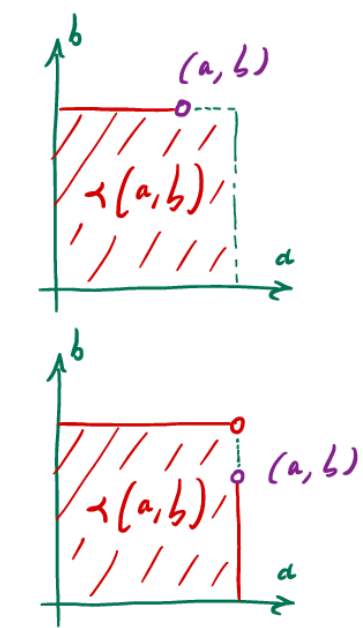
\includegraphics[width=2.5cm]{immagini/ordine_omega.png}
	\end{wrapfigure}
	Che è lo stesso ordinamento che abbiamo usato per dimostrare che il prodotto di numerabili è numerabile.
	\textcolor{MidnightBlue}{In pratica, per confrontare $(a,b)$ con $(a',b')$, si confrontano prima $\max(a,b)$ e $\max(a',b')$;
	a parità si confrontano $a$ e $a'$; se anche queste coincidono, si confrontano $b$ e $b'$.}\\
	Abbiamo già verificato, nella dimostrazione di $\aleph_0^2 = \aleph_0$, che $\prec$ è un buon ordine (con $\omega$ al posto di $\omega_\alpha$, ma le verifiche sono identiche\footnote{Tranne nel caso del buon ordinamento in cui bisogna fare un'induzione transfinita su $\alpha$ per coprire il caso di intersezione non vuota.}).
	Resta da verificare che vale proprio:
	\[ X \Mydef (\omega_\alpha \times \omega_\alpha, \prec) \sim \omega_\alpha
		\]
	Sia $\beta$ l'ordinale corrispondente a $X$, dobbiamo mostrare, per avere l'isomorfismo di buoni ordinamenti, che i cardinali sono uguali, ovvero $\beta = \omega_\alpha$. Siccome $|\omega_\alpha| \leq |\omega_\alpha \cdot \omega_\alpha| = |\beta|$, e $\omega_\alpha$ è iniziale, per la contronominale della definizione di ordinali
	iniziale otteniamo che $\beta \geq \omega_\alpha$, dunque non dobbiamo far altro che escludere che $\omega_\alpha < \beta$, ovvero che $\omega_\alpha$ non è isomorfo ad un segmento iniziale proprio di $X$.\\
	Fissiamo un segmento iniziale proprio $X_{(a,b)}$ di $X$ e dimostriamo che $|X_{(a,b)}| < \aleph_\alpha$, cioè si avrebbe che $|X_{(a,b)}| < |\omega_\alpha|$ e quindi non può accadere che $X_{(a,b)} \sim \omega_\alpha$.\\
	Sia $\mu := \max(a,b)$, essendo $a,b \in \omega_\alpha$, si ha naturalmente che $\mu < \omega_\alpha$ e $\omega_\alpha$ è iniziale, quindi limite, si ha $s(\mu) < \omega_{\alpha}$, e di nuovo $|s(\mu)| < \aleph_\alpha$. Di conseguenza, per la monotonia della funzione degli aleph, $|s(\mu)| = \aleph_\gamma$, per qualche $\gamma < \alpha$, oppure $s(\mu) \in \omega$.
	\begin{itemize}
		\item Nel primo caso $|s(\mu) \times s(\mu)| = \aleph_\gamma^2 \overset{\text{\textcolor{orange}{Hp. indutt.}}}{=} \aleph_\gamma$.
		\item Nel secondo caso $s(\mu) \times s(\mu)$ è finito, e quindi $|s(\mu) \times s(\mu)| < \aleph_0$.
	\end{itemize}
	In ogni caso $|s(\mu) \times s(\mu)| < \aleph_\alpha$ e, siccome vale che $X_{(a,b)} \subseteq s(\mu) \times s(\mu)$, abbiamo allora $|X_{(a,b)}| \leq |s(\mu) \times s(\mu)| < \aleph_\alpha$, come voluto. \hfill $\square$

\begin{exercise}
	Per $n \in \omega$ sia $\ps^n(X) \Mydef \{Y \in \ps(X) : |Y| = n\}$, dimostrare che $\forall n \in \omega$ si ha che $|\ps^n(\omega_\alpha)| = \aleph_\alpha$.
\end{exercise}

\begin{soln}
	Possiamo definire la seguente mappa:
	\[ \omega_\alpha \hookrightarrow \ps^n(\omega_\alpha) : x \mapsto \Imm(f_x)
		\]
	dove:
	\[ f_x : n \to \omega_\alpha : i \mapsto f_x(i) = \begin{cases}
		x &\text{se $i = 0$} \\
		x + i &\text{se $1 \leq i \leq n - 1$}
	\end{cases}
		\]
	Osserviamo in primis che $f_x$ è iniettiva per ogni $x \in \omega_\alpha$, dunque $n = |\Imm(f_x)| \in \ps^n(\omega_\alpha)$, e quindi la mappa sopra è ben definita, infatti $f_x(i) = f_x(j) \to x + i = x + j$,
	e per la stretta monotonia nella seconda componente della somma ordinale si ha $i = j$. Da quanto appena detto segue anche che le funzioni $f_x$ sono strettamente crescenti,
	dunque se $\Imm(f_x) = \Imm(f_y)$, poiché sono insiemi finiti, per cui bene ordinati, ed isomorfi a $n$, l'isomorfismo possibile è uno solo, per un fatto noto, ed è quello definito ricorsivamente che manda ogni volta un elemento 
	nel minimo elemento dell'insieme d'arrivo più grande di tutti quelli dell'immagine ristretta, per cui si ha proprio $f_x = f_y$, da cui $x = f_x(0) = f_y(0) = y$. Abbiamo quindi ottenuto che $\aleph_\alpha = |\omega_\alpha| \leq |\ps^n(\omega_\alpha)|$.\\
	Viceversa, possiamo definire la mappa:
	\[ \ps^n(\omega_\alpha) \to \omega_\alpha^n : A \mapsto (a_0,\ldots,a_{n-1})
		\]
	con $a_i$, $i$-esimo elemento di $A$, ordinato secondo l'ordine di $\omega_\alpha$ ristretto ad $A$. Naturalmente tale mappa è ben definita, visto che ogni insieme produce esattamente una $n$-upla, ed è iniettiva in quanto due $n$-uple uguali implicano tutti
	gli elementi uguali e quindi gli insiemi uguali.\footnote{Questa stessa idea, leggermente modificata per risolvere il problema nel caso $\ps^{\leq n}(\omega_\alpha)$.}
\end{soln}

\begin{exercise}
	Dimostrare che $\psf(\omega_\alpha) = \aleph_\alpha$.\footnote{\textbf{\underline{Hint}}: Osservare che $|$sottoinsiemi finiti di $\omega_\alpha| \leq |\{f : n \to \omega_\alpha | n \in \omega\}|$ [\textcolor{red}{Typo Mamino}], fissare $g : \omega_\alpha \times (\omega_\alpha \sqcup \{\spadesuit\}) \to \omega_\alpha \sqcup \{\spadesuit\}$ biunivoca e definire
	$h : \{f : n \to \omega_\alpha | n \in \omega\} \to \omega_\alpha$ con $h(\emptyset) = \spadesuit$ e $h(f) = g(f(0),h(x \mapsto f(x+1)))$.}
\end{exercise}

\begin{soln}
	Dal basso naturalmente abbiamo la mappa $\omega_\alpha \hookrightarrow \psf(\omega_\alpha) : x \mapsto \{x\}$, che ci dà $\aleph_\alpha \leq |\psf(\omega_\alpha)|$. Per la disuguaglianza opposta, in primis definiamo la mappa:
	\[ \psf(\omega_\alpha) \to \{f \in {}^n \omega_\alpha | n \in \omega\} = \bigcup_{n \in \omega} {}^n\omega_\alpha : A \mapsto f_A
		\]
	dove:
	\[ f_A : m = |A| \to \omega_\alpha : x \mapsto \min\{y \in \omega_\alpha | x \in  A \land y > f_A[x]\}
		\]
	ed osserviamo che poiché le $f_A$ sono strettamente crescenti (in particolare $|A| \in \omega$ ed $A \subseteq \omega_\alpha$ sono bene ordinati, dunque c'è un unico isomorfismo tra loro, ed è quello in cui mappiamo $A$),
	allora $f_A = f_B \implies \Imm(f_A) = \Imm(f_B) \implies A = B$, dunque la mappa è iniettiva ed abbiamo la disuguaglianza $|\psf(\omega_\alpha)| \leq |\{f \in {}^n \omega_\alpha | n \in \omega\}|$. Osserviamo ora che, fissata una
	bigezione $g : \omega_\alpha \times (\omega_\alpha \sqcup \{\spadesuit\}) \to \omega_\alpha \sqcup \{\spadesuit\}$, possiamo definire la mappa:
	\[ h : \{f \in {}^n \omega_\alpha | n \in \omega\} \to \omega_\alpha \cup \{\spadesuit\} : f \mapsto \begin{cases}
		\spadesuit &\text{se $f = \emptyset$} \\
		g(f(0),h(f(x + 1))) &\text{altrimenti}
	\end{cases}
		\]
	che è naturalmente ben definita (grazie a $g$) ed iniettiva, infatti, se abbiamo che $h(f) = h(f')$ in arrivo, o $f = f' = \emptyset$ oppure $g(f(0),f(x+1)) = g(f'(0),f'(x+1))$, che, per la bigettività di $g$, implica $f(0) = f'(0)$ e $h(f(x+1)) = h(f'(x+1))$, che, ripetendo il ragionamento,
	implica a sua volta $f(1) = f'(1)$, e $h(f(x+2)) = h(f'(x+2))$, e così via, ottenendo $f(i) = f'(i)$, $\forall 0 \leq i \leq n-1$, da cui $f = f'$ ed abbiamo l'iniettività. Abbiamo quindi ottenuto che $|\psf(\omega_\alpha)| \leq |\omega_\alpha \sqcup \{\spadesuit\}| = \aleph_\alpha + 1 = \aleph_\alpha$\footnote{L'ultima
	uguaglianza è vera senza AC e la si può ottenere sfruttando disuguaglianze oppure il fatto che $\omega \hookrightarrow \omega_\alpha$.}.
\end{soln}

\begin{exercise}
	Dimostrare che $\forall \alpha,\beta \in \Ord$ si ha:
	\[ |\alpha| = |\beta| = \aleph_\gamma \to |\alpha + \beta| = |\alpha \cdot \beta| = |\alpha^{\beta}| = \aleph_\gamma 
		\]
	dove intendiamo la cardinalità delle tre operazioni ordinali.
\end{exercise}

\begin{soln}
	Per la monotonia [debole] delle operazioni ordinali nella prima componente si ha $\alpha \leq \alpha + \beta, \alpha \cdot \beta, \alpha^\beta$, da cui si ottiene la disuguaglianza dal basso 
	in tutti e tre i casi, $\aleph_\gamma = |\alpha| \leq |\alpha + \beta|, |\alpha \cdot \beta|, |\alpha^\beta|$. Per il viceversa, vediamo caso per caso:
	\begin{itemize}
		\item $\alpha + \beta = \alpha \sqcup \beta$, per cui $|\alpha + \beta| = |\alpha \sqcup \beta| = |\alpha| + |\beta| = \aleph_\gamma + \aleph_\gamma = \aleph_\gamma$.
		\item $\alpha \cdot \beta = \alpha \times \beta$, per cui $|\alpha \cdot \beta| = |\alpha \times \beta| = |\alpha| \cdot |\beta| = \aleph_\gamma \cdot \aleph_\gamma = \aleph_\gamma$.
		\item $\alpha^\beta = \{f \in {}^\alpha\beta : \; |\supp(f)| < \aleph_0\} \subseteq \psf(\alpha \times \beta)$, per cui $|\alpha^\beta| \leq |\psf(\alpha \times \beta)| = |\psf(\omega_\gamma \times \omega_\gamma)| = |\psf(\omega_\alpha)| = \aleph_\gamma$,
		dove l'uguaglianza tra la cardinalità dele parti finite è indotta dalla bigezione tra gli insiemi (basta fissare una bigezione e poi definire quella tra gli insiemi mandando ogni elemento delle prime parti finite nella sua immagine tramite la prima bigezione),
		mentre l'ultima uguaglianza è l'esercizio precedente.
	\end{itemize}
\end{soln}

\begin{exercise}
	Se $|X| = \aleph_\alpha$ e $f : X \to Y$ è una funzione, allora $|f[X]| \leq \aleph_\alpha$.
\end{exercise}

\begin{soln}
	Possiamo assumere, a meno di bigezione, che $X = \omega_\alpha$ e definire la funzione:
	\[ g : f[X] \to X : y \mapsto \min_<(f^{-1}(y))
		\]
	che è naturalmente ben definita ed è iniettiva perché stiamo considerando i minimi di una partizione di $X$, dunque due minimi sono uguali se e solo se consideriamo lo stesso elemento della partizione di $X$, cioè la stessa controimmagine,
	da cui si ottiene, applicando $f$, che in partenza i valori devono essere uguali.
\end{soln}

\begin{exercise}
	Dimostrare che $\forall \alpha \; \in \Ord \; \aleph_{\alpha + 1} < 2^{2^{\aleph_\alpha}}$.
\end{exercise}

\begin{soln}
	Poiché per Cantor si ha $\aleph_\alpha < 2^{\aleph_\alpha}$, essendo per definizione ricorsiva della funzione degli aleph, che $\aleph_{\alpha + 1}$ è il più piccolo ordinale iniziale infinito strettamente maggiore di $\aleph_\alpha$, si ha $\aleph_{\alpha + 1} \leq 2^{\aleph_\alpha}$.
	Infine si osserva che $\aleph_{\alpha} \leq 2^{\aleph_\alpha} < 2^{2^{\aleph_\alpha}} \to \aleph_{\alpha} < 2^{2^{\aleph_\alpha}}$.
\end{soln}